\section{Non-parametric regression}

\subsection{Report Bandwidth Corresponding to Minimum Estimated Risk}

After running the Nadaraya-Watson kernel regression using the Epanechnikov and Gaussian kernel and performing cross-validation for bandwidth selection, the optimal bandwidth corresponding to the minimum estimated risk is:


\begin{itemize}
	\item Optimal Bandwidth of \textbf{Gaussian} kernel: 0.180
	\item Optimal Bandwidth of \textbf{Epanechnikov} kernel: 0.164
\end{itemize}


\subsection{Similarities and Differences Due to Choice of Different Kernel Functions}

\subsubsection{Similarities}
\begin{itemize}
	\item \textbf{General Functionality:} Both kernels assign weights to
	      data points based on their distance from the query point, resulting
	      in similar predictions in regions with high data density.
	\item \textbf{Smoothing:} As the bandwidth increases, all kernel
	      functions produce smoother estimates. At very large bandwidths, all
	      kernels oversmooth the data, giving too much influence to distant
	      points.
	\item \textbf{Cross-validation Behavior:} Both kernels display a
	      similar behavior during cross-validation, and the corresponding
	      risk curves follow the same trend with bandwidth changes.
\end{itemize}

\subsubsection{Differences}
\begin{itemize}
	\item \textbf{Shape of the Weights:}
	      \begin{itemize}
		      \item \textbf{Epanechnikov Kernel:} This kernel assigns
		            zero weight to points farther than the bandwidth due
		            to its quadratic form, creating a more localized
		            effect.
		      \item \textbf{Gaussian Kernel:} This kernel assigns
		            non-zero weight to every point, regardless of
		            distance, due to its exponential decay. It results in
		            smoother estimates, but it is more sensitive to
		            distant points.
	      \end{itemize}

	\item \textbf{Sensitivity to Outliers:}
	      \begin{itemize}
		      \item \textbf{Epanechnikov Kernel:} This kernel is more
		            resilient to outliers because they assign zero or
		            reduced weight to distant points, decreasing the
		            influence of outliers on the prediction.
		      \item \textbf{Gaussian Kernel:} The Gaussian kernel is
		            more prone to incorporating outliers, as it assigns
		            non-zero weights even to far-away points, making it
		            less resilient in the presence of outliers.
	      \end{itemize}
	\item \textbf{Plots}
	      \begin{itemize}
		      \item \textbf{Epanechnikov Kernel:} This kernel produces
		            more precise and localized estimates, with a good
		            balance between bias and variance when using the
		            optimal bandwidth.
		      \item \textbf{Gaussian Kernel:} The Gaussian kernel leads
		            to smoother curves but gives undue influence to
		            distant points, which can result in overfitting or
		            oversmoothing depending on the bandwidth.
	      \end{itemize}
\end{itemize}
\begin{figure}[H]
	\centering
	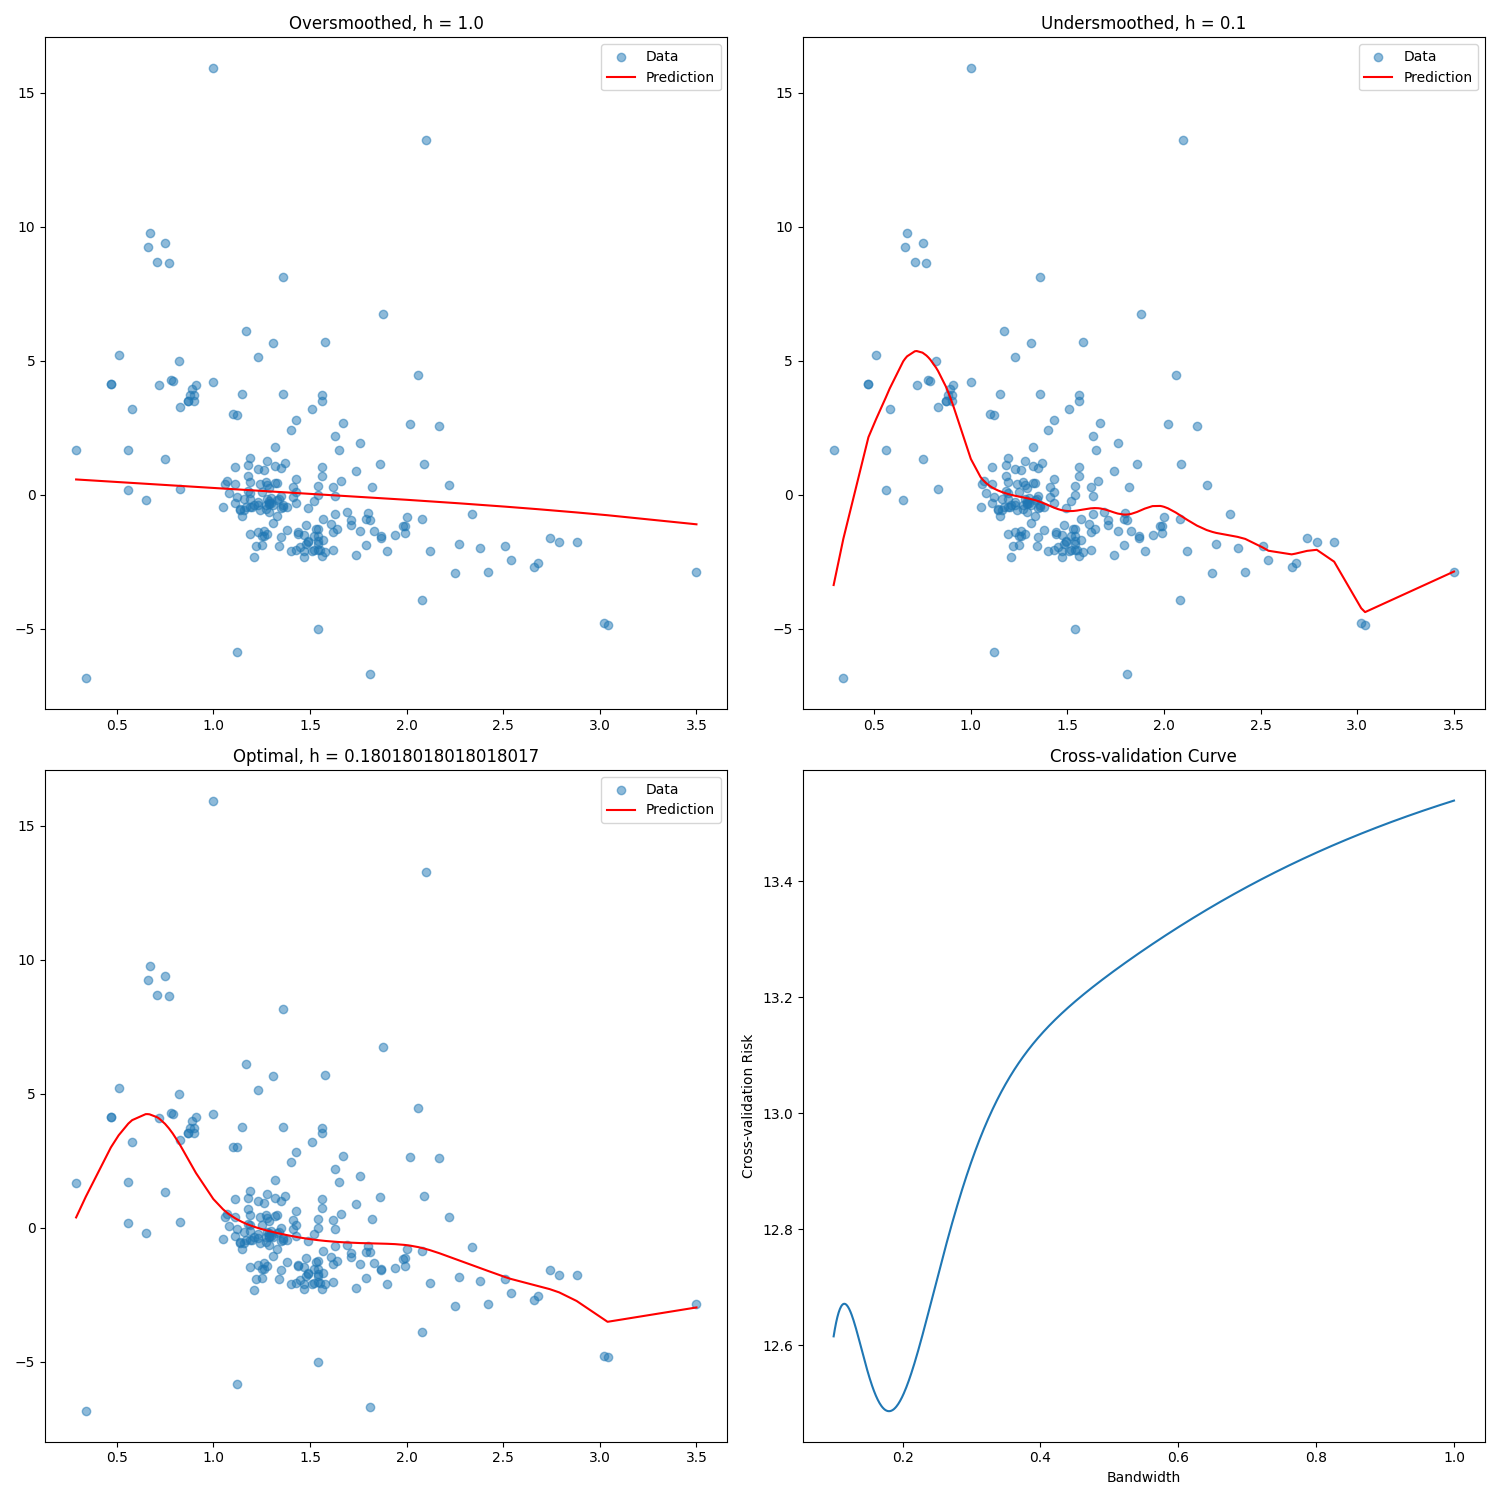
\includegraphics[width=0.5\textwidth]{../images/4/gaussian_kernel_regression.png}
	\caption{Oversmoothed, undersmoothed, optimal and cross validation curve of gaussian kernel}
\end{figure}

\begin{figure}[H]
	\centering
	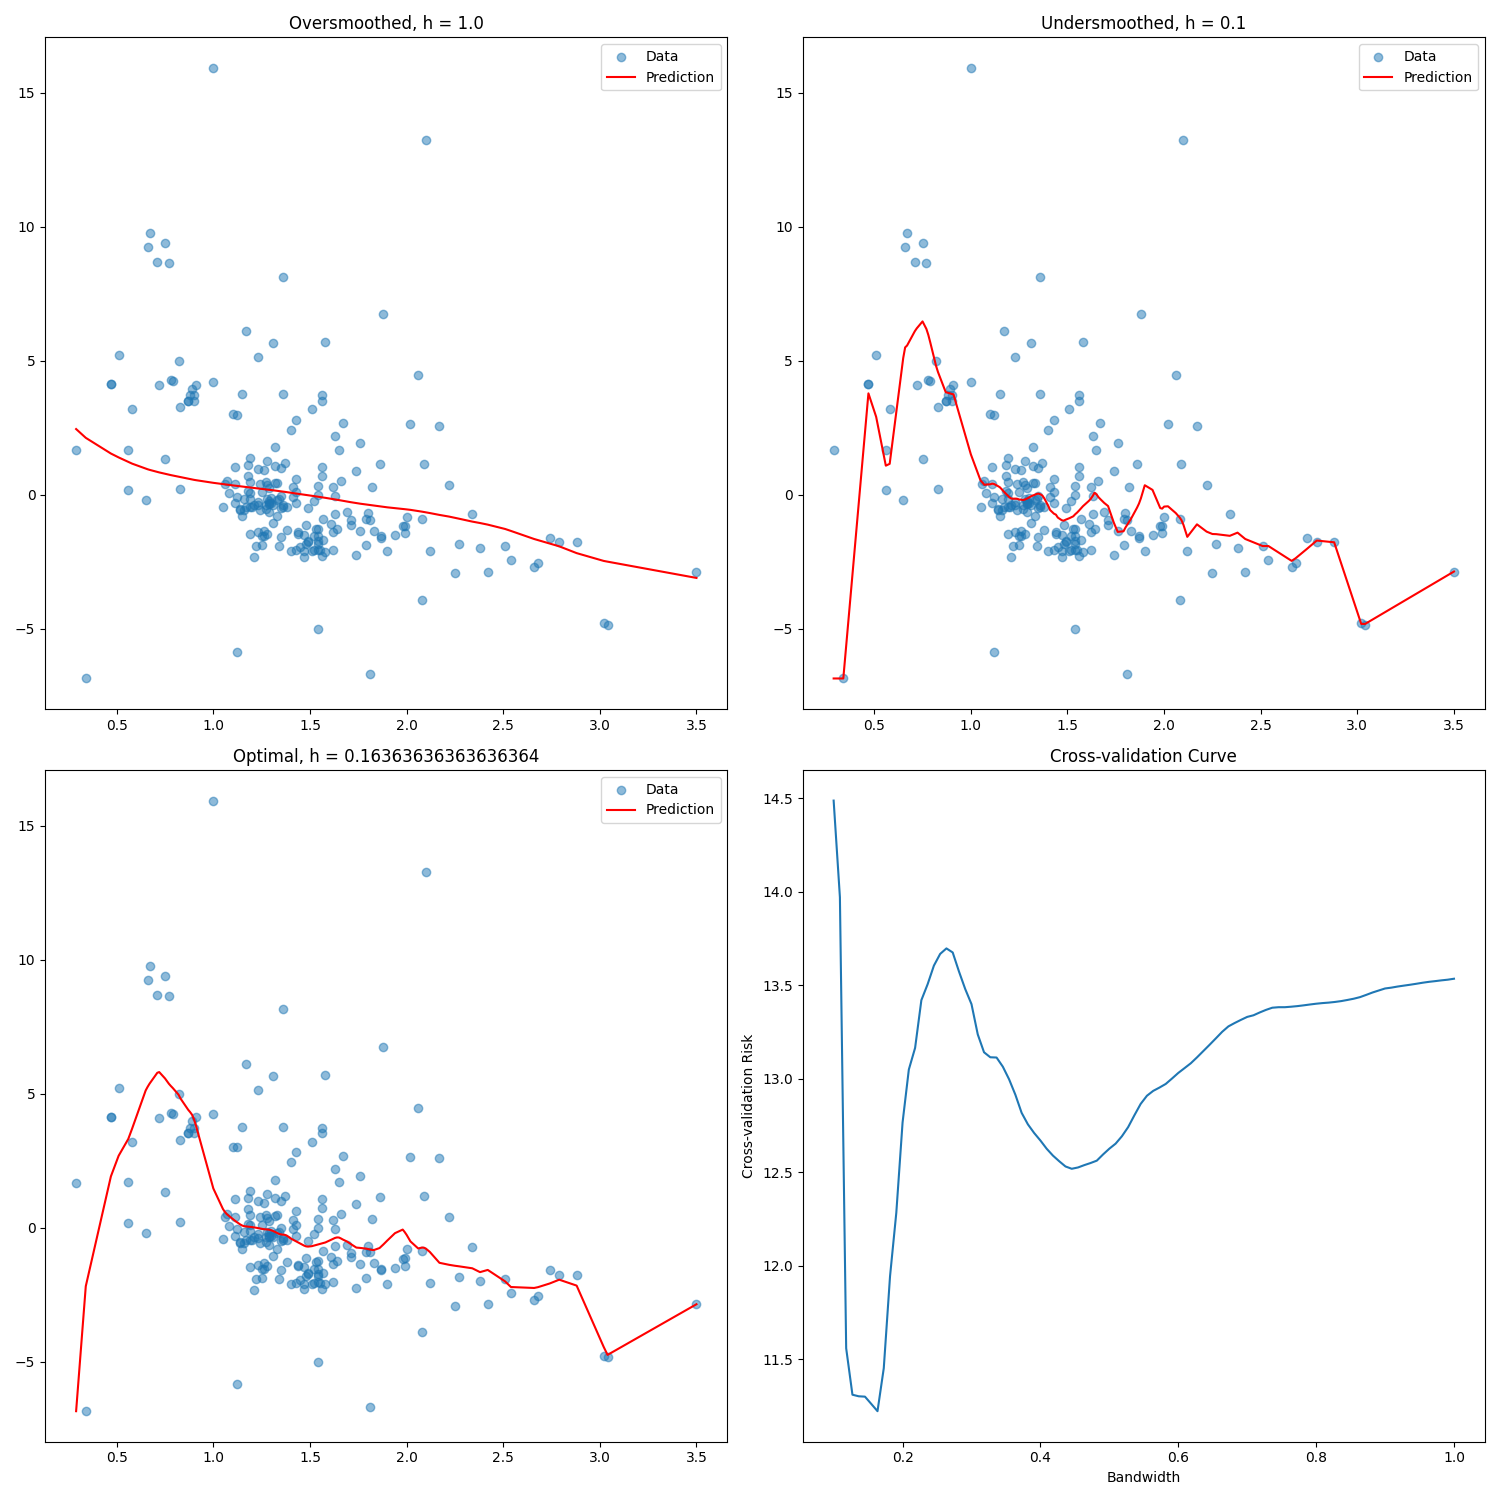
\includegraphics[width=0.5\textwidth]{../images/4/epanechnikov_kernel_regression.png}
	\caption{Oversmoothed, undersmoothed, optimal and cross validation curve of epanechnikov kernel}
\end{figure}
